\documentclass[a4paper]{article}
\usepackage{graphicx,amsmath,amssymb,hyperref,url,color,multirow}
\usepackage{cases}
\usepackage{ulem}
\usepackage{epstopdf}
\usepackage{listings}
\usepackage{float}
\usepackage{subcaption}
\usepackage{algorithmicx}
\usepackage{algorithm}
\usepackage[noend]{algpseudocode}
\usepackage[section]{placeins}
\usepackage[super]{nth}

\title{Ideas}
\date{}

\begin{document}

\maketitle


%\begin{abstract}
%% Target submission: https://www.computer.org/csdl/journal/ts/about/14409?title=About&periodical=IEEE%20Transactions%20on%20Software%20Engineering
%
%%Possible relevant related work: 
%% https://www.computer.org/csdl/journal/ts/2019/12/08345680/13rRUxNEqRR
%% https://www.computer.org/csdl/journal/ts/1981/04/01702851/13rRUwI5TYT
%% https://onlinelibrary.wiley.com/doi/pdf/10.1111/j.1937-5956.2009.01025.x?casa_token=3jvWXTriMngAAAAA:4WjMvJ43VYTeQ6dwDSI2ZVFza5t69kaQPCLg0LkDLH9njkd0DImnhza6I_F8MQ_L7KkUsP1PGocudt69
%% http://sutlib2.sut.ac.th/sut_contents/H131799.pdf
%% https://www.researchgate.net/profile/Ahmed_E_Hassan/publication/276835606_Continuously_mining_distributed_version_control_systems_an_empirical_study_of_how_Linux_uses_Git/links/578e604a08ae81b4466ec59c/Continuously-mining-distributed-version-control-systems-an-empirical-study-of-how-Linux-uses-Git.pdf
%% https://www.usenix.org/legacy/event/nsdi06/tech/full_papers/yip/yip.pdf
%
%% https://dl.acm.org/doi/pdf/10.1145/2568225.
%
%% https://par.nsf.gov/servlets/purl/10063078
%
%%software performance and scalability
%	
%The software development process continuously evolves triggered by the changes either in organizational practices or development practices. The produced code goes through several phases before being merged in the upstream. Over time, several of these phases have been optimized and automatized, most recently using Agile techniques and the supporting Continuous Integration (CI) automation infrastructure. However, a model that would enable studying the process is currently missing. In this paper, we propose a queuing theory model for the software testing and integration process. Our model empowers analysis and optimization of staff or infrastructure allocation. We show that the model can be used to analyse and optimize along several dimensions, including by reducing the overload on the persons who review and merge the code, by shrinking the size of the team, increasing the number of persons authorized to merge, re-engineering how the infrastructure is scaled or the way the tests are written and run. 
%
%Our experimental results also demonstrate that; i) there are two developer activity peaks in any day, one before the lunch break and the second towards the end of the work day, and ii) the probability of developer to commit a code follows an exponential distribution.
%
% 
%
%
%\end{abstract}
%
%%% Keywords. The author(s) should pick words that accurately describe
%%% the work being presented. Separate the keywords with commas.
%\keywords{model, software testing, software integration, process, queuing theory, arrival rate, peak hour activity, optimization, development process, infrastructure, tests}
%
%
\section{Questions and Answers}

-- in that paper for which you reproduced the results, the idea is that executing tests in cloud environments is trivial and there are infinite resources available. However, doing it on embedded devices needs careful infrastructure pre-planning to optimize investments and costs and that's what the model is useful for. 


-- However, in reality many companies end up paying quite some money for various SaaS and cloud bills. There are start-ups that try to help keeping track of such expenses: https://www.cleanshelf.com   So the question is: can we use the model to predict cloud infrastructure costs for various developer team sizes and test execution times? For instance consider on-demand instance pricing: https://aws.amazon.com/ec2/pricing/on-demand/   What are the costs on a regular month, what about when one has a deadline? Infrastructure cost vs human time cost tradeoff. 


-- Even broader - how many optimization dimensions do we have along which we could analyze: team size, test execution time, [Would you be able to make a list with them?]? The discussion section below (Sec 7) tries to do a bit of that but it's not strong enough.

\subsection{Q1: What are the infrastructure costs in normal working periods vs periods with deadlines?}
Something like: assuming a developer team of 20 people, average test execution time of 5 mins, average test wait time 5 mins how many units of cost U would a company spend per month to ensure various GoS 90, 95, 98, 100 \%?  (let's first talk about units of costs in an abstract way, then map to various on-demand instance costs).
\newline \textbf{Answer:}
First I calculated a number of servers that are required to achieve the desired grade of service. I calculated them for two different cases: in case there is a deadline and in case there is no deadline.
In the case where there is no deadline (Figure \ref{no_deadline}), I assumed that each developer would make commits 3 times a day. In case there is a deadline (Figure \ref{deadline}), I assumed that each developer commits 9 times per day.
I calculated the average number of hours per day that the servers are used. In our model it is about 10 hours per day. I don't think that this is very relevant, because we simulate the whole process with the same parameters, which in reality only apply to a peak hour.

\begin{table}
\begin{tabular}{ c c c  c }
& 1 deadline/week & 2 deadlines/week & 3 deadlines/week \\ \hline
 GoS $90\%$ & 680 & 760& 840 \\ 
 GoS $95\%$& 680 & 760 & 840\\  
 GoS $98\%$ & 880 & 960 & 1040 \\
 GoS $100\%$ & 3280 & 3560 & 3840 \\
\end{tabular}
\caption{Let the cost of servers be 1 U/hour. In the table we have monthly costs in U for 20 working days}
\end{table}

\begin{figure}[h!]
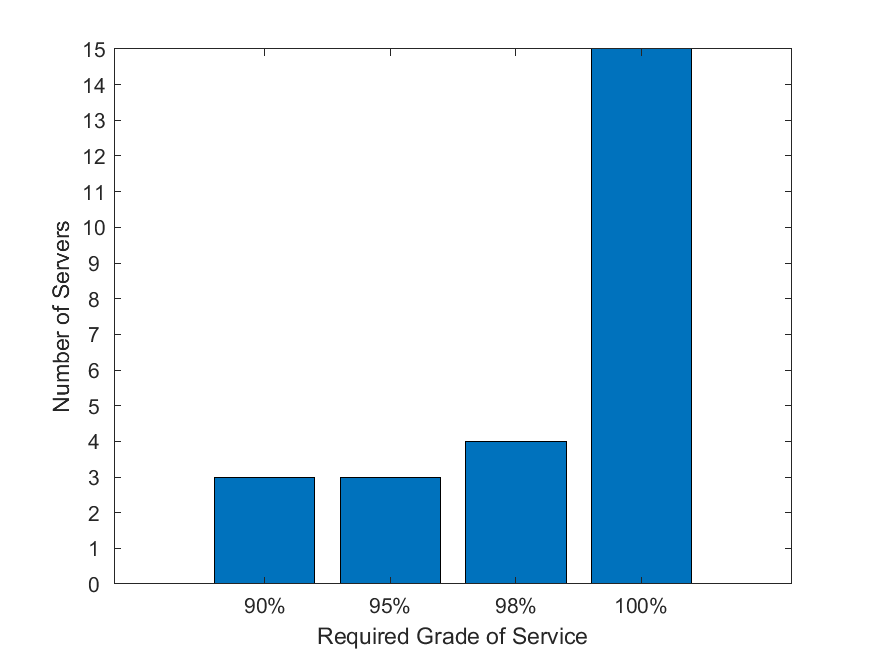
\includegraphics[scale=0.7]{plots/Question1_nodeadline.png}
\caption{Number of required servers in order to achieve desired grade of service.}
\label{no_deadline}
\end{figure}  

\begin{figure}[h!]
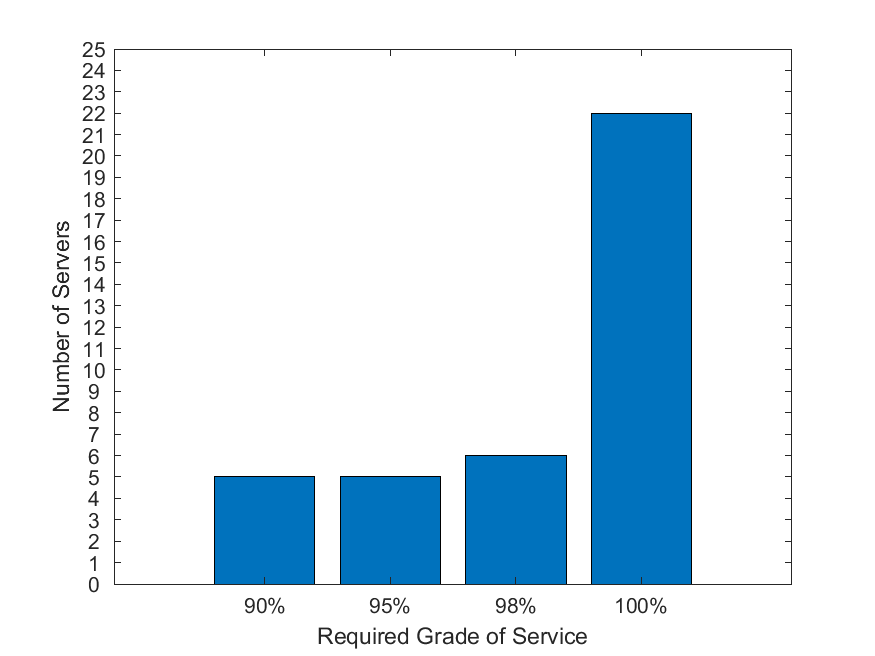
\includegraphics[scale=0.7]{plots/Question1_deadline.png}
\caption{Number of required servers in order to achieve desired grade of service.}
\label{deadline}
\end{figure}  

\subsection{Q2: What are the infrastructure costs for various teams of various sizes?}
Along the lines we discussed that for 300 devs you need N servers, but for 10x30 devs you likely need less than N servers all other params being the same.

\noindent \textbf{Answer:} Parameters used in Figure \ref{300_one_team}:
\begin{itemize}
\item number of developers $k = 300$
\item average testing time $h = 3$ minutes
\item acceptable waiting time $w = 10$ minutes
\item number of commits per day per developer $r = 3$
\item percent of commits in a peak hour $p = 0.1$
\end{itemize}

\begin{figure}[h!]
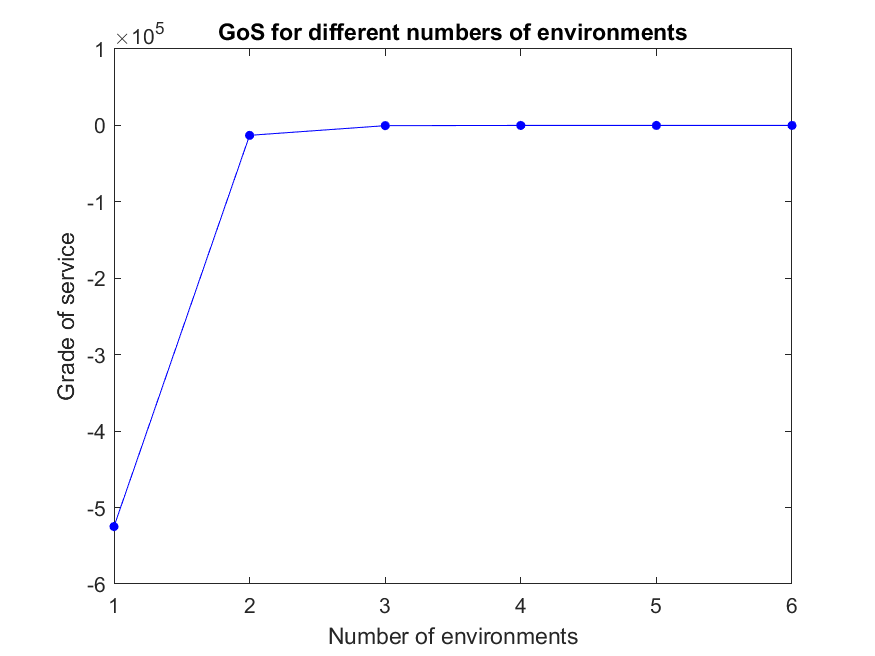
\includegraphics[scale=0.7]{plots/Grade_of_service_300_developers.png}
\caption{Grades of service for different $N$ and 300 developers in one team}
\label{300_one_team}
\end{figure}  
For $N=6$, the grade of service is $99.72 \% $. If we devide the developers into 10 teams of 30 developers each, we have several different options:
\begin{enumerate}
\item All teams share the servers: In this case we can easily see that the situation is exactly the same as before, because there are 300 individual developers using N servers, just as before. The teams play no role here. 
\item Each team has its own servers: In  Figure \ref{30_one_team} we see that for grade of service greater than $99 \%$, a team of 30 developers needs 2 servers. If each team has its own servers and doesn't share them with another team, then we need 20 servers, which is much more than in the first case.
\item It is also possible for a team to have a few servers to itself and share some servers with others. If we devide 300 developers into 10 teams of 30 developers each, we can immediately see that we are not getting the optimal solution. Each team needs at least 1 server for itself, so we already need 10 servers and don't even have the required grade of service.
\end{enumerate}

\begin{figure}[h!]
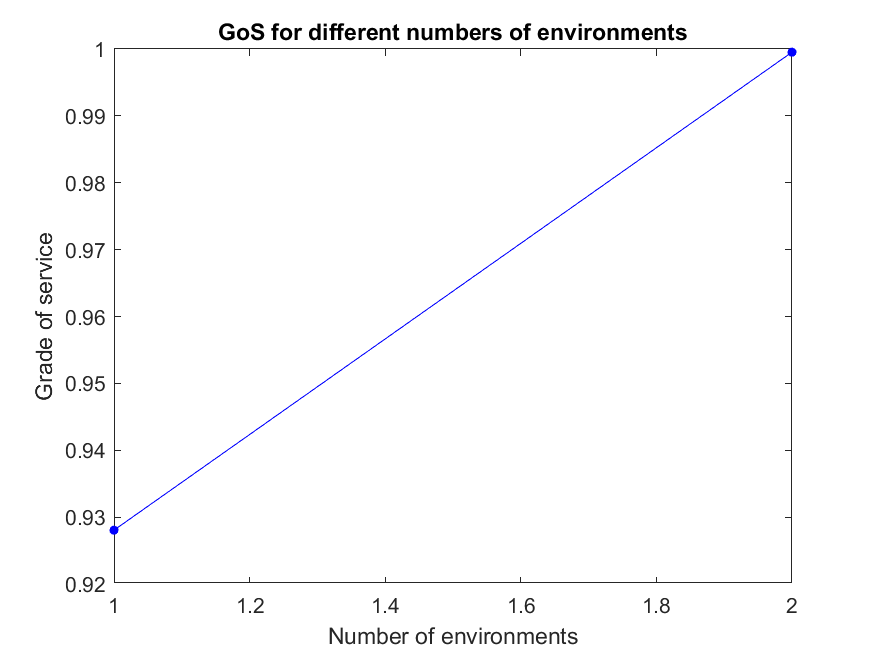
\includegraphics[scale=0.7]{plots/Grade_of_service_30x10_developers.png}
\caption{Grades of service for different $N$ and 30 developers in one team}
\label{30_one_team}
\end{figure} 

\noindent These results are actually quite to be expected. If each team has servers for itself and doesn't have to share them with another team, it can happen that in some teams some servers are free and in other teams there is a long queue of commits waiting to be tested.

\noindent There is another related interesting question: if one of the development teams has much longer average testing time, is it better for this team to have its own servers, or is it better to share them with other developers?
I have simulated this situation. There are 200 developers who share the servers, and it takes an average of 3 minutes to run tests for them. For the required grade of service of $95\%$ we need 4 servers. 
\newline We also have another team of 100 developers, whose tests take 10 minutes on average. For the required grade of service of $95\%$ we need 7 servers. The acceptable waiting time is 10 minutes for both teams. 

\textit{I simulated this situation and got some results. However, I don't quite know how to visualise them. I got similar results as before: for required GoS we (on average) need less servers when everybody is sharing them. }

\subsection{Q3: How does the way the tests are engineered affect the development process?}
How does the way the tests are engineered affect the development process in terms of waiting times, in terms of cost units for infrastructure, in terms of cost units for people waiting?


\subsection{Optimization dimensions:}
\begin{itemize}
\item team size
\item execution time
\item number of environments (required GoS)
\item deadlines/no deadlines

\end{itemize}
\end{document}